\section{Lemme de \textsc{Lebesgue}}

\todoinline{Parvenir à décommenter le marginnote suivant. D'après mes recherches sur internet, il faudrait "externaliser" la compilation des figures en pdflatex qui demandent trop de ressources.}

\begin{lemme}
% \marginnote[0cm]{Source : \cite{maths-france} Planche no 37. Intégration sur un segment}
Soit $a < b$.
\begin{enumerate}
\item On suppose que $f$ est une fonction de classe $\mathscr{C}^1$ sur $[a, b]$. Alors,
\[
\lim_{ \lambda \to +\infty} \int_a^b \sin(\lambda t) f(t) \d t = 0.
\]

\item Redémontrer le même résultat en supposant simplement que la fonction $f$ est continue par morceaux sur~$[a, b]$.
\end{enumerate}
\end{lemme}

\todoinline{
Ajout du graphique suivant, à supprimer ou améliorer en coloriant les aires positives et négatives ?
}

\todoarmand{Je suis partant pour laisser le graphique, j'ai ajouté une version avec les aires colorées.}

On constate sur la figure suivante que plus $\lambda$ est grand, plus les oscillations sont élevées et plus les aires comptées positivement et négativement se compensent.
\begin{center}
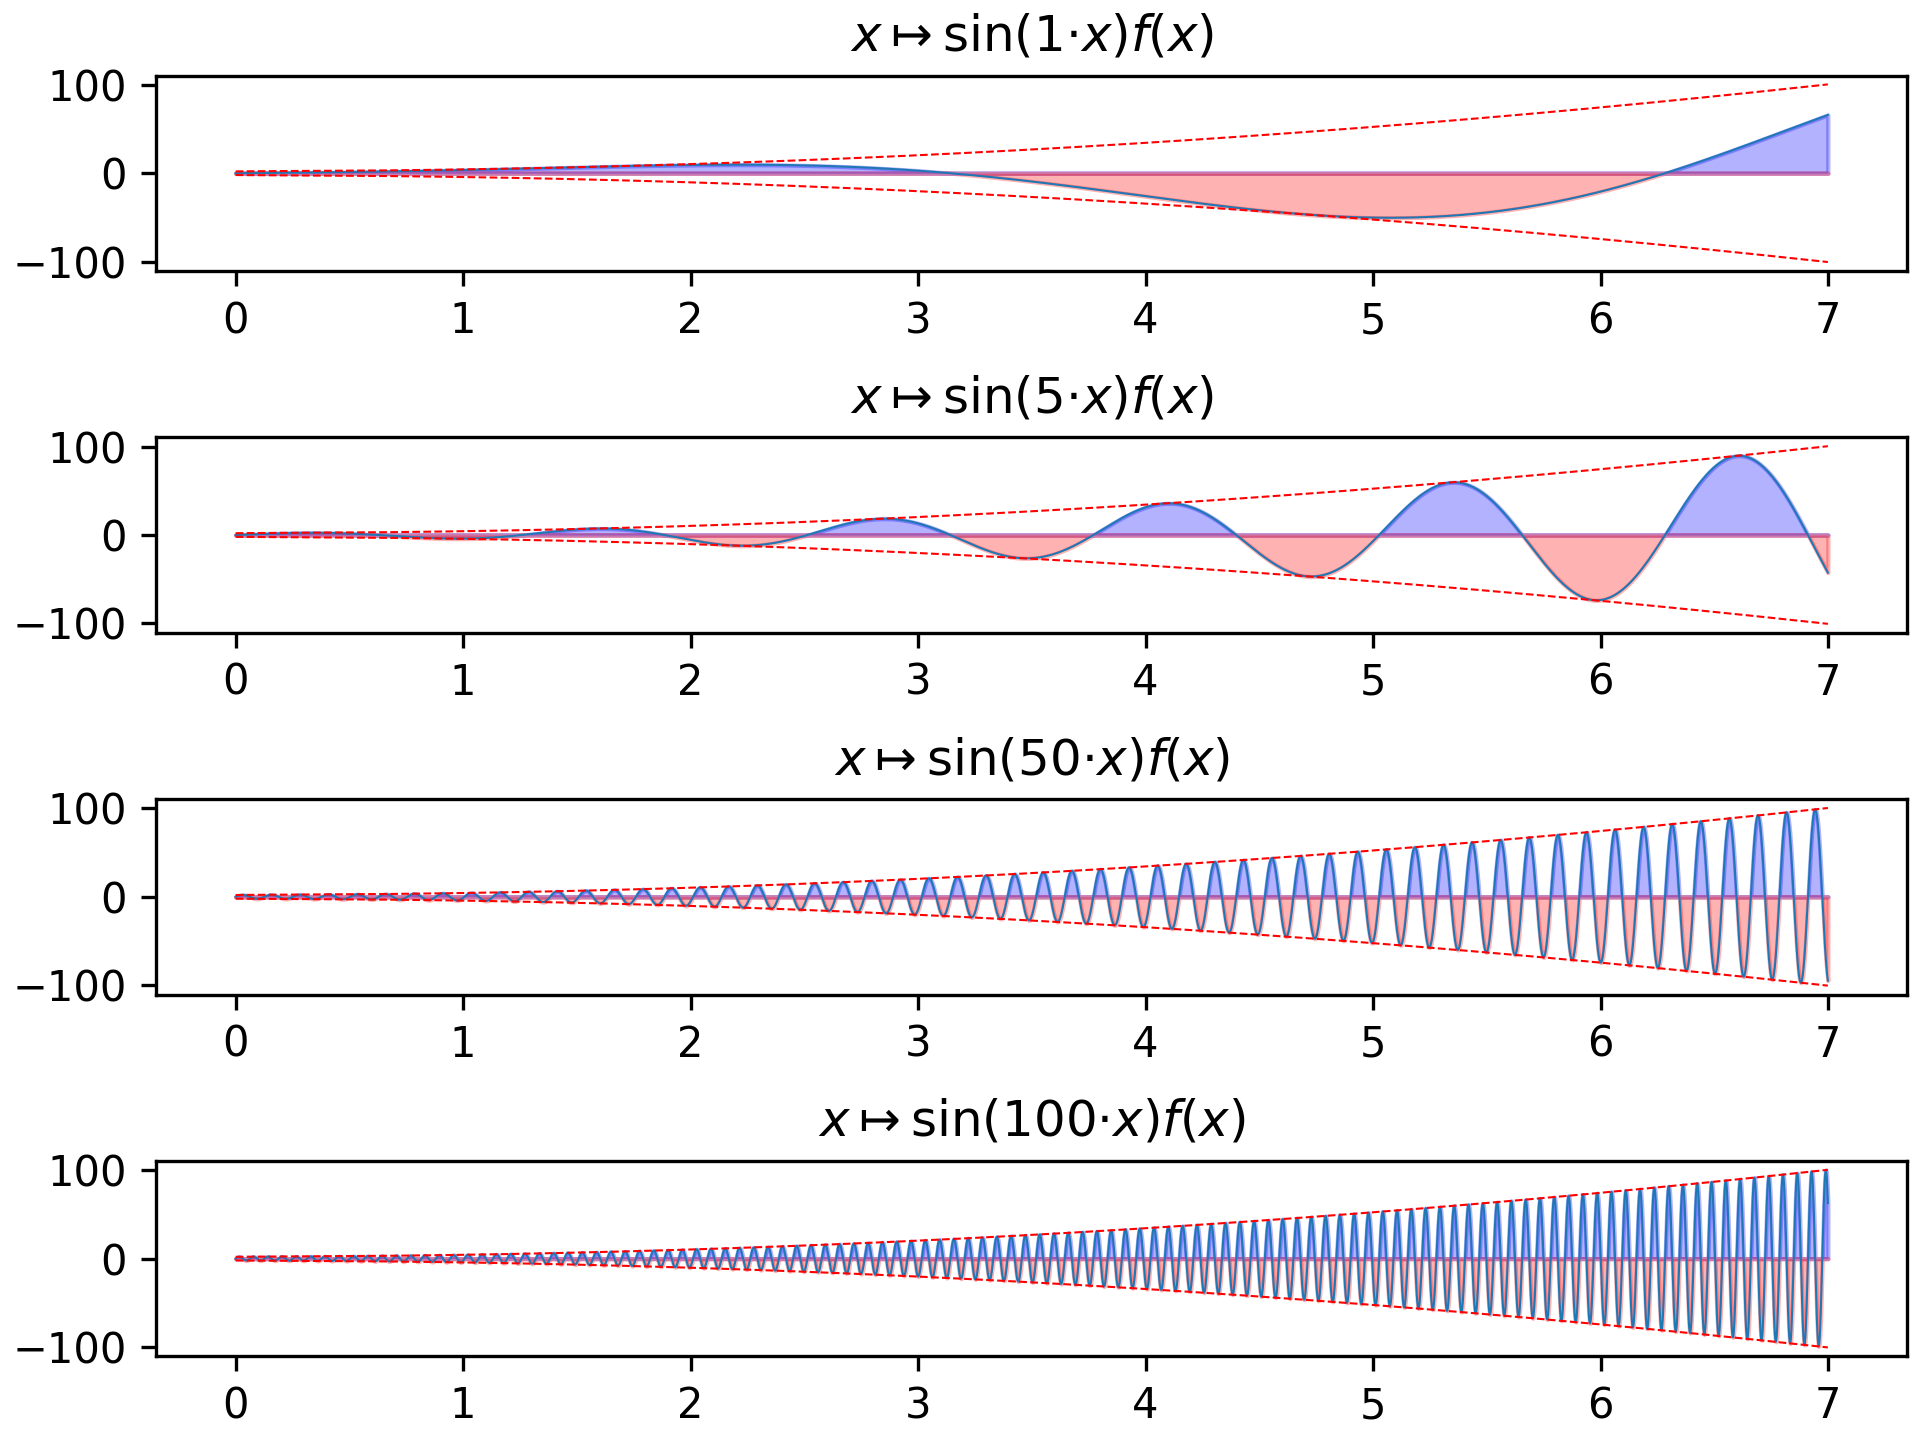
\includegraphics[width=0.75\textwidth]{illustrations/integration-02_lebesgue.png}
\end{center}

\begin{solution}
    \begin{enumerate}
        \item Puisque la fonction $f$ est de classe $\mathscr{C}^1$ sur $[a, b]$, on peut effectuer une intégration par parties qui fournit pour $\lambda > 0$:
        $$\left| \int_a^b f(t) \sin(\lambda t) \d t \right| = \left| \frac{1}{\lambda} \left( -\big[ \cos(\lambda t) f(t) \big]_a^b + \int_a^b f'(t) \cos(\lambda t) \d t  \right) \right| \leqslant \frac{1}{\lambda} \left( |f(a)| + |f(b)| + \int_a^b |f'(t)| \d t \right).$$
        Cette dernière expression tend vers $0$ quand $\lambda$ tend vers $+ \infty$, et donc $\int_a^b f(t) \sin(\lambda t) \d t$ tend vers $0$ quand $\lambda$ tend vers $+\infty$.
        \item Si la fonction $f$ est simplement supposée continue par morceaux, on ne peut donc plus effectuer une intégration par parties. \\
        Le résultat est clair si $f = 1$, car pour $\lambda > 0$, $\left| \int_a^b \sin(\lambda t) \d t \right| = \left| \frac{\cos(\lambda a) - \cos(\lambda b)}{\lambda} \right| \leqslant \frac{2}{\lambda}$. \\
        Le résultat s'étend aux fonctions constantes par linéarité de l'intégrale puis aux fonctions constantes par morceaux par additivité par rapport à l'intervalle d'intégration, c'est-à-dire aux fonctions en escaliers. Pour toute fonction $g$ continue par morceaux sur $[a, b]$, on note $\|g\|_{\infty} = \sup_{[a, b]} |g|$.\\
        Soit alors $f$ une fonction continue par morceaux sur $[a, b]$. \\
        \todoinline{Là on admet un théorème d'approximation non trivial et hors programme en PCSI. Il faut voir ce qu'on indique en introduction du chapitre ?}
        Soit $\varepsilon > 0$. Il existe une fonction en escalier $\varphi$ telle que $\|f - \varphi\|_\infty \leq \varepsilon$. De plus, d'après le point précédent, il existe un réel $\lambda_0$ strictement positif tel que pour tout $\lambda > \lambda_0$,
        \[
        \left|\int_a^b \sin(\lambda t) \varphi(t) \d t\right| \leq \varepsilon.
        \]
        Finalement, d'après l'inégalité triangulaire, pour tout $\lambda > \lambda_0$,
        \begin{align*}
        \left|\int_a^b f(t) \sin(\lambda t) \d t\right|
        &\leq         \left|\int_a^b (f(t) - \varphi(t)) \sin(\lambda t) \d t\right| + \left|\int_a^b \varphi(t) \sin(\lambda t) \d t\right|\\
        &\leq \norme{f - \varphi}_\infty (b - a) + \varepsilon\\
        &\leq \varepsilon (1 + b - a).
        \end{align*}
Finalement, $\lim\limits_{\lambda \to +\infty} \int_a^b f(t) \sin(\lambda t) \d t = 0$.
        \end{enumerate}
\end{solution}


% \todoinline{
% La variante proposée ci-dessous me semble difficile.
%
% Le calcul de $\sum \frac{1}{n^2}$ est classique et pourrait être directement généralisé avec St Cyr 1995 - Je mets une version dans le dossier /chapitres/integration/documents. En plus on ferait un peu de polynômes de Bernoulli.
%
% Le calcul de l'intégrale de Dirichlet est top.
% }

% \todoarmand{Cela me convient, nous pouvons supprimer la variante. On pourrait la remplacer par le  mais en renvoyant vers un exercice du chapitre polynômes.}

\bigskip


\todoinline{Ajouter des liens dans le texte ci-dessous.}

Nous allons utiliser le lemme de Lebesgue pour calculer certaines valeurs de la fonction $\zeta$ de Riemann. Nous verrons ultérieurement une autre utilisation au calcul de la valeur de l'intégrale de Dirichlet.

\todoinline{Partie re-rédigée, à relire !}

\todoinline{Citer sujet St Cyr 1995}

\todoinline{Faire référence à une section sur $\zeta$ et une section sur Bernoulli}

\todoinline{Dans la partie sur Bernoulli, il faudra :
la symétrie, la dérivée et les valeurs de $B_2(0)$ et $B_4(0)$}

On note $(B_n)$ la suite des polynômes de Bernoulli et, pour tout $x > 1$, $\zeta(x) = \sum\limits_{k=1}^{+\infty} \frac{1}{k^x}$.

\begin{theo}
Pour tout $m \geq 1$, $\zeta(2m) = (-1)^{m-1} (2 \pi)^{2m} \frac{B_{2m}(0)}{2}$.
\end{theo}

On rappelle que 
\begin{align*}
B_n(1 - x) &= (-1)^n B_n(x),\\
B_n'(x) &= n B_{n-1}(x).
\end{align*}

\begin{elem_sol}
Pour $k$ et $n$ entiers strictement positifs, on défnit:
\[
I_{n, k} = \int_0^1 B_n(t) \cos(2 k \pi t) \d t.
\]

\begin{enumerate}
\item Pour tout entier $p > 0$,
\[
I_{2p, k} = \frac{(-1)^{p-1}}{(2 k \pi)^{2p}} \quad \text{et} \quad I_{2p+1,k} = 0.
\]

En effet, en utilisant deux intégrations par parties successives,
\[
I_{n,k} = \frac{1}{4k^2 \pi^2} \big(B_{n-1}(1) - B_{n-1}(0) - I_{n-2, k} \big).
\]
De plus, $I_{0,k} = 0$, $I_{1,k} = 0$, $I_{2,k} = \frac{1}{4 \pi^2}$? Donc,
\[
\forall n \geqslant 3,\, I_{n,k} = - \frac{1}{4 k^2 \pi^2}I_{n-2, k}.
\]
On obtient ainsi le résultat annoncé
\end{enumerate}

Pour tout entier naturel $n$ strictement positif, on pose:
\[
\forall t \in \interoo{0}{1}, \quad \varphi_n(t) = \frac{B_n(t) - B_n(0)}{\sin(\pi t)}.
\]

\begin{enumerate}[resume]
\item Pour tout $n \geq 2$, la fonction $\varphi_n$ est prolongeable par continuité à $\interff{0}{1}$ et que le prolongement est de classe $\mathscr{C}^1$. En effet,

\begin{itemize}
\item D'après les quotients de fonctions de classe $\mathscr{C}^1$ dont le dénominateur ne s'annule pas, la fonction $\varphi_n$ est de classe $\mathscr{C}^1$ sur $\interoo{0}{1}$.

\item La fonction $B_n$ étant polynomiale, elle est de classe $\mathscr{C}^1$ en $0$ et, en utilisant la formule de \textsc{Taylor}--\textsc{Young},
\begin{align*}
\varphi_n(t) &= \frac{B'_n(0)t + \frac{B''_n(0)}{2}t^2 + o(t^2)}{\pi t \big(1 + o(t) \big)} \\
&= \frac{B'_n(0)}{\pi} + \frac{B''_n(0)}{2 \pi}t + o(t).
\end{align*}

Ainsi, $\lim\limits_0 \varphi_n = \frac{B'_n(0)}{\pi}$ et $\varphi_n$ est une fonction prolongeable par continuité en $0$.

\item
% De plus, $\lim\limits_{t \to 0} \frac{\varphi_n(t) - \frac{B'_n(0)}{\pi}}{t} = \frac{B''_n(0)}{2 \pi}$.
%
De plus, pour tout $t$ non nul, $\varphi'_n(t) = \frac{B'_n(t) \sin(\pi t) - \big(B_n(t) - B_n(0) \big) \pi \cos(\pi t)}{\sin(\pi t)^2}$. Ainsi, en effectuant un développement limité à l'ordre $2$ du numérateur, alors $\lim\limits_{t \to 0} \varphi'_n(t) = \frac{1}{2 \pi} B''_n(0)$.

D'après le théorème de prolongement des dérivées, $\varphi_n$ est prolongeable en une fonction de classe $\mathscr{C}^1$ sur $\interfo{0}{1}$.

Enfin, $\varphi_n(1-t) = (-1)^n \frac{B_n(t) - B_n(1)}{\sin(\pi t)}$. Comme, pour tout $n \geqslant 2$, $B_n(0) = B_n(1)$, alors la fonction $\varphi_n$ est bien prolongeable en une fonction de classe $\mathscr{C}^1$ sur $\interff{0}{1}$.
\end{itemize}
\end{enumerate}

Pour tout $N$ entier naturel non nul et $t \in \interoo{0}{1}$, on pose :
\[
D_n(t) = 1 + 2 \sum_{k=1}^N \cos(2k \pi t) = \frac{\sin\big((2N+1) \pi t \big)}{\sin(\pi t)}.
\]

\begin{enumerate}[resume]
\item Cette quantité, appelée noyau de Dirichlet, s'exprime simplement à l'aide de la fonction sinus :
\[
D_n(t) = \frac{\sin\big((2N+1) \pi t \big)}{\sin(\pi t)}.
\]
En effet, pour tout $t \in \interoo{0}{1}$, $\e^{2 \i k \pi t} \not= 1$. Ainsi, d'après la somme des termes d'une suite géométrique, 
    \begin{align*}
        \sum_{k=0}^N \e^{2 \i k \pi t} &= \frac{\e^{2 \i (N+1) \pi} - 1}{\e^{2 \i \pi} - 1} \\
        &= \e^{\i N \pi} \frac{\sin(N+1) \pi t}{\sin(\pi t)}. \\
        \sum_{k=0}^N \cos(2 k \pi t) &= \cos(N \pi t) \frac{\sin \big((N+1) \pi t \big)}{\sin(\pi t)}\text{, en prenant les parties réelles,} \\
        1 + 2 \sum_{k=1}^N \cos(2 k \pi t) &= 2 \frac{\cos(N \pi t) \sin \big((N+1) \pi t\big)}{\sin(\pi t)} - 1 \\
        &= \frac{\sin\big((2N+1) \pi t \big) + \sin( \pi t)}{\sin(\pi t)} - 1 \\
        &= \frac{\sin\big((2N+1) \pi t \big)}{\sin(\pi t)}.
    \end{align*}

\item Ainsi,
\[
\int_0^1 \varphi_{2m}(t) \sin \big((2N+1) \pi t \big) \d t
= - B_{2m}(0) + 2 \sum_{k=1}^N \frac{(-1)^{m-1}}{(2 k \pi)^{2m}}.
\]

En effet, d'après la définition de $\varphi_{2m}$,
\begin{align*}
\int_0^1 \varphi_{2m}(t) \sin \big((2N+1) \pi t \big) \d t &= \int_0^1 \big(B_{2m}(t) - B_{2m}(0) \big) \frac{\sin\big((2N+1) \pi t \big)}{\sin(\pi t)} \d t \\
&= \int_0^1 \big( B_{2m}(t) - B_{2m}(0) \big) \d t + \cdots \\
&\cdots + 2 \sum_{k=1}^N \int_0^1 \big(B_{2m}(t) - B_{2m}(0) \big) \cos(2 k \pi t) \d t \\
&= - B_{2m}(0) + 2 \sum_{k=1}^N \frac{(-1)^{m-1}}{(2 k \pi)^{2m}}.
\end{align*}

\item D'après le lemme de Lebesgue,
\[
\lim_{N\to+\infty} \int_0^1 \varphi_{2m}(t) \sin \big((2N+1) \pi t \big) \d t = 0
\]
et on obtient bien le résultat annoncé.
\end{enumerate}
\end{elem_sol}


\begin{remarque}
En utilisant les valeurs remarquables des premiers polynômes de Bernoulli, on obtient
\begin{align*}
\sum_{k=1}^{+\infty} \frac{1}{k^2} &= 2 \pi^2 B_2(0) = \frac{\pi^2}{6} \\
\sum_{k=1}^{+\infty} \frac{1}{k^4} &= -2^3 \pi^4 B_4(0) = \frac{\pi^4}{90}.
\end{align*}
\end{remarque}